%%%%%%%%%%%% Attribution %%%%%%%%%%%%
% This template was created by 
% Chuck F. Rocca at WCSU and may be
% copied and used freely for 
% non-commercial purposes.
% 10-17-2021
%%%%%%%%%%%%%%%%%%%%%%%%%%%%%%%%%%%%%

%%%%%%% Start Document Header %%%%%%%
% In creating a new document
% copy and paste the header 
% as is.
%%%%%%%%%%%%%%%%%%%%%%%%%%%%%%%%%%%%%
\documentclass[12pt]{article}

\usepackage{tikz} 
\usepackage{geometry}
\usepackage{listings}
\usepackage{pdfpages}
\usepackage{hyperref}
\usepackage{minted}
\usepackage{booktabs}
\hypersetup{
    colorlinks=true,
    linkcolor=blue,
    filecolor=magenta,      
    urlcolor=cyan,
    pdftitle={Overleaf Example},
    pdfpagemode=FullScreen,
    }

\urlstyle{same}
\geometry{margin=1in}
%%%% Header Information %%%%

%%%% Document Information %%%%
    \title{RME 3111 - Lab 2: Heap}
    \author{
    Course Instructor: Dr. Sejuti Rahman\\
    \\
    Md. Arban Hossain (SH-092-005)\\
    }
    \date{10 Feb 2023}

%%%%%%% End Document Header %%%%%%%


%%%% Begin Document %%%%
% note that the document starts with
% \begin{document} and ends with
% \end{document}
%%%%%%%%%%%%%%%%%%%%%%%%

\begin{document}

%%%% Format Running Header %%%%%

%%%% Insert the Title Information %%%
\maketitle


%%%% Introduction to the General Template %%%%
\section*{The A* Algorithm}
The A* algorithm is an informed search algorithm that uses a heuristic function to guide the search. The heuristic function is used to estimate the cost of the path from the current vertex to the destination. It is guaranteed to find the shortest path if the heuristic function is admissible. An admissible heuristic function is one that never overestimates the cost of the path from the current vertex to the destination.

\[ h(n) \leq d(n) \]
\noindent
Here,

$h(n)$ = The heuristic cost of the path from the vertex to destination

$d(n)$ = The actual cost of the path from the vertex to destination

\noindent
If the original cost to reach a node from the source is denoted by $g(n)$, the modified cost for the node will be,

\[f(n) = g(n) + h(n)\]

We can then run uniform cost search on the modified graph. At each step, we dequeue a node from the \textbf{Priority Queue} and check the neighbor nodes that can be reached immediately from it. If a neighbor node has a node cost that is greater than the cost of the current node plus the cost of the edge between them, we update the cost of the neighbor node and push it into the Priority Queue. We continue this process until have dequeued the destination node.

\pagebreak


Consider the following directed graph. The vertices are labeled with their names and the edges are labeled with their costs.

\begin{center}
  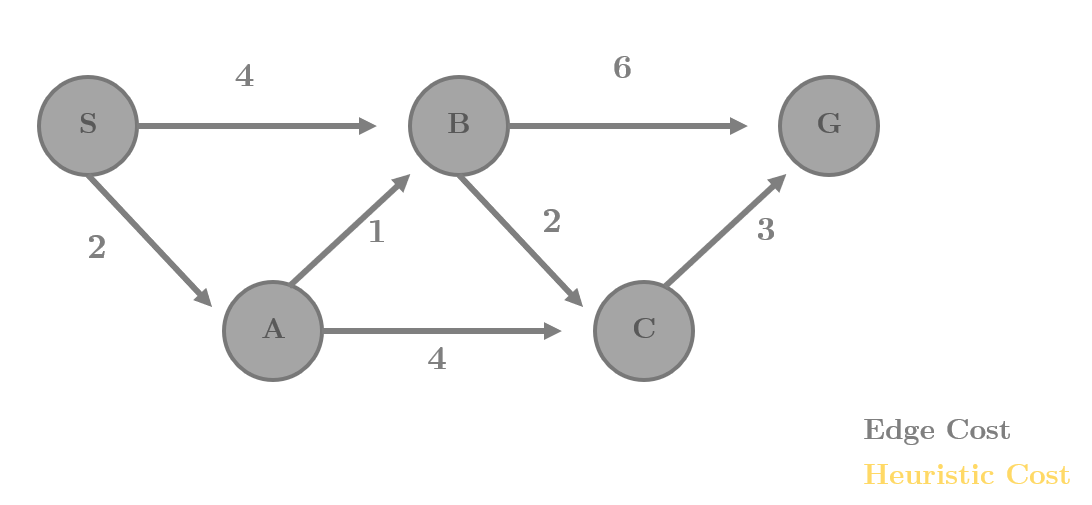
\includegraphics[width=0.9\textwidth]{Graph.png}
\end{center}

% \section*{Pen and Paper Simulation}

\subsection*{Heuristic 1}

For the following set of heuristics, we can simulate the search process manually.

% A horizontal table containing 2 rows, one for the vertex name and the other for the heuristic cost.

\begin{table}[h]
  \centering
  \begin{tabular}{cc}
  \toprule
  \textbf{Vertex} & \textbf{Heuristic Cost} \\
  \midrule
  S & 8 \\
  A & 3 \\
  B & 7 \\
  C & 2 \\
  G & 0 \\
  \bottomrule
  \end{tabular}
\end{table}


% Add images of heuristic1_Page 1 to 6

\begin{center}
  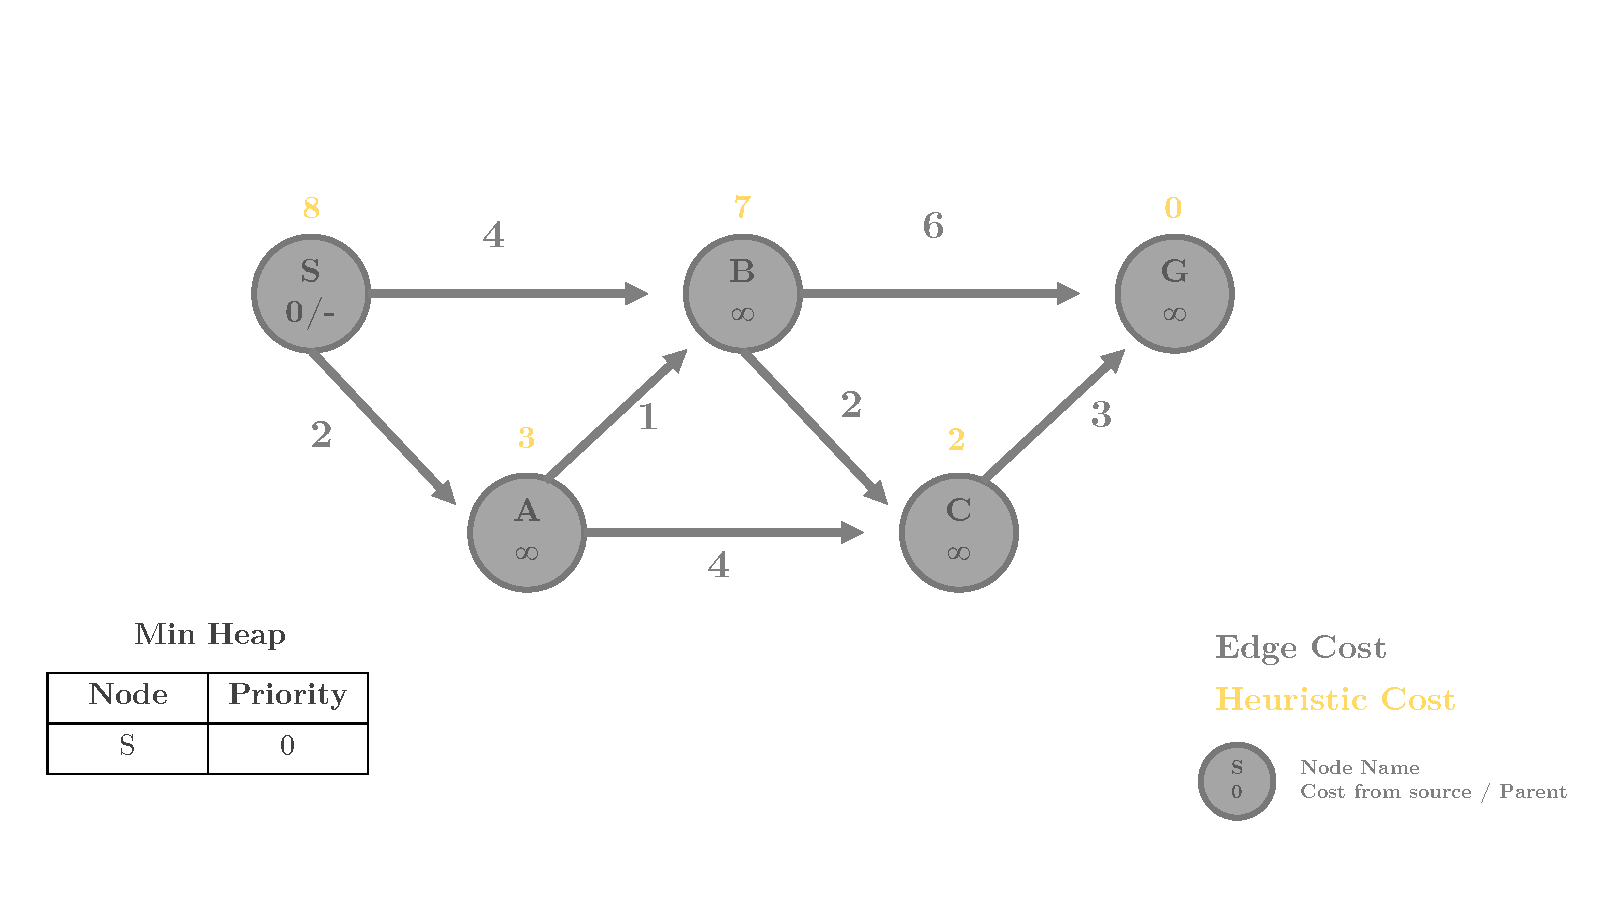
\includegraphics[width=0.8\textwidth]{heuristic1_Page1.png}
\end{center}

\begin{center}
  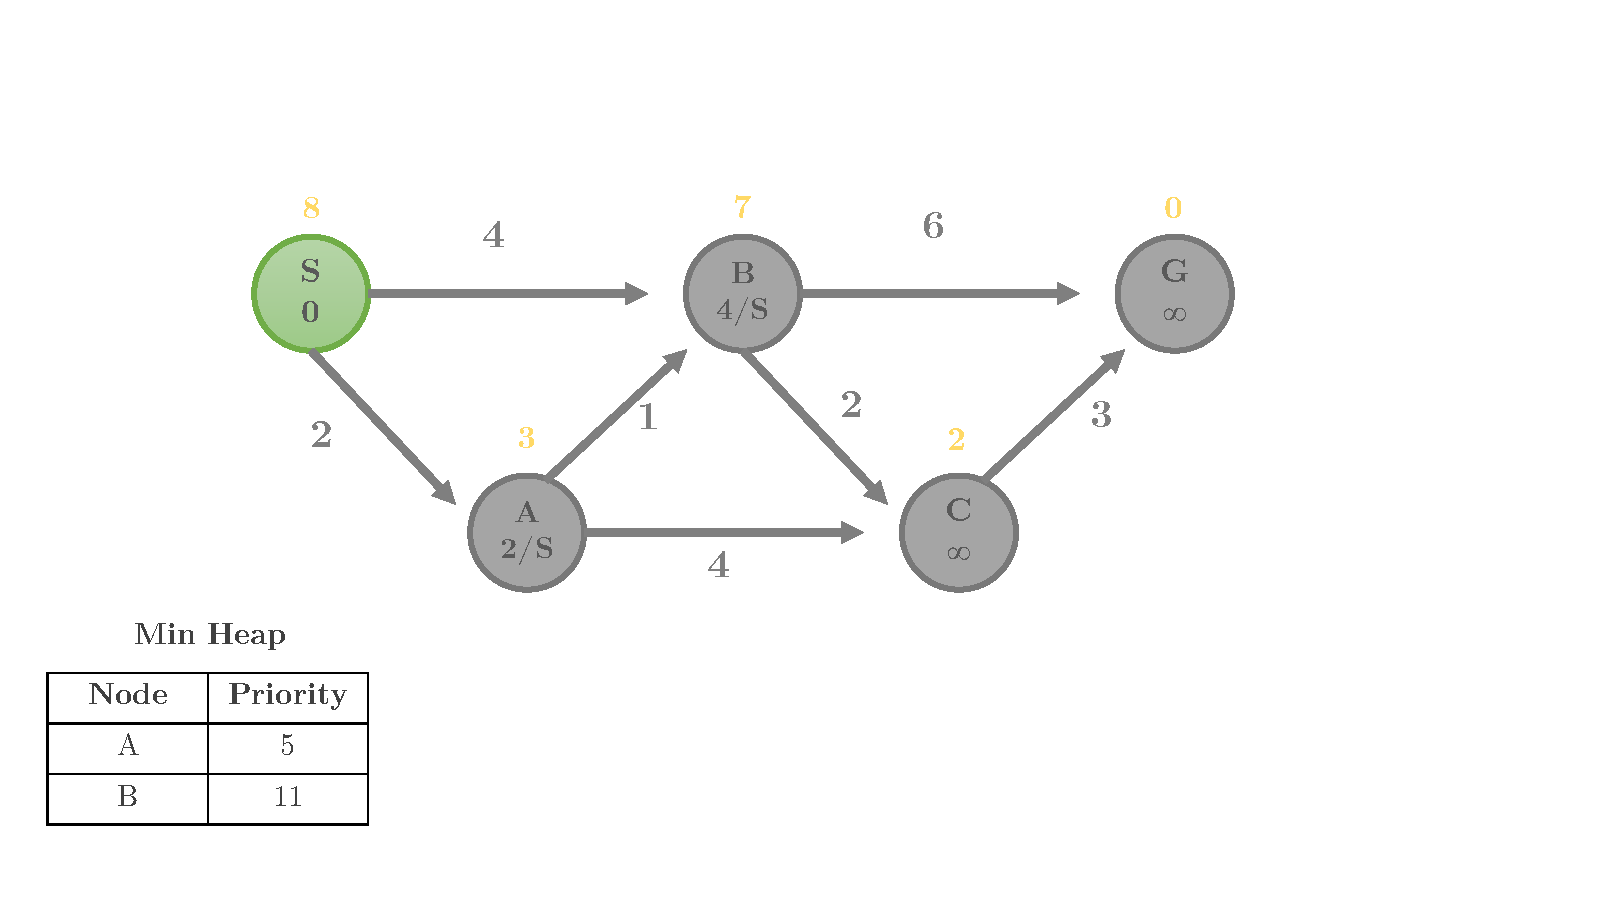
\includegraphics[width=0.9\textwidth]{heuristic1_Page2.png}
\end{center}

\begin{center}
  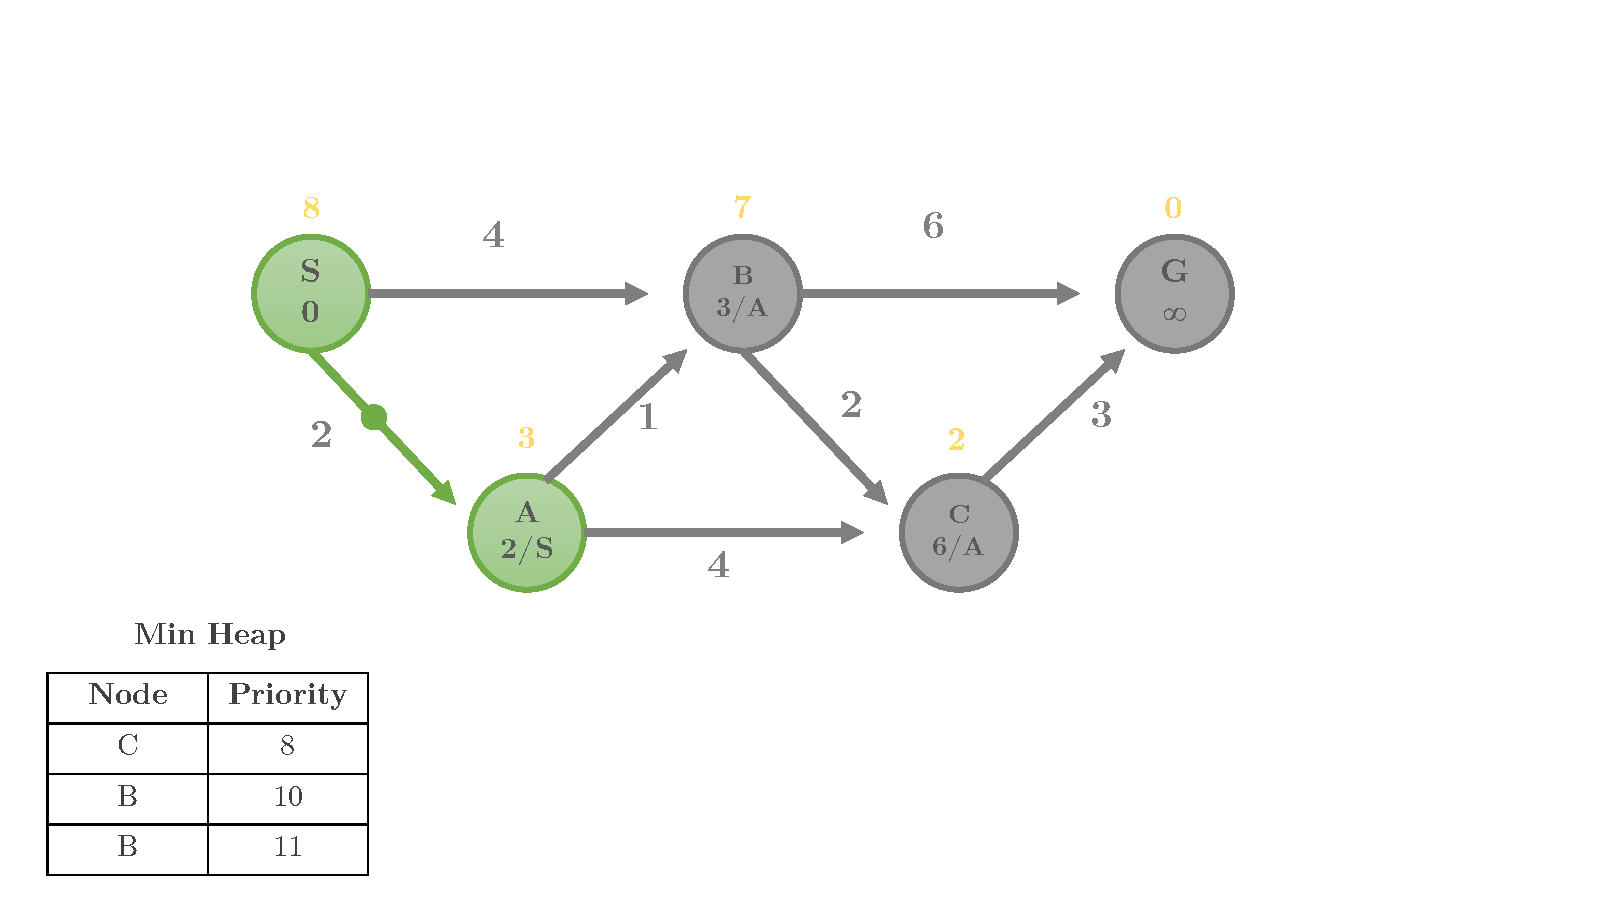
\includegraphics[width=0.9\textwidth]{heuristic1_Page3.png}
\end{center}

\begin{center}
  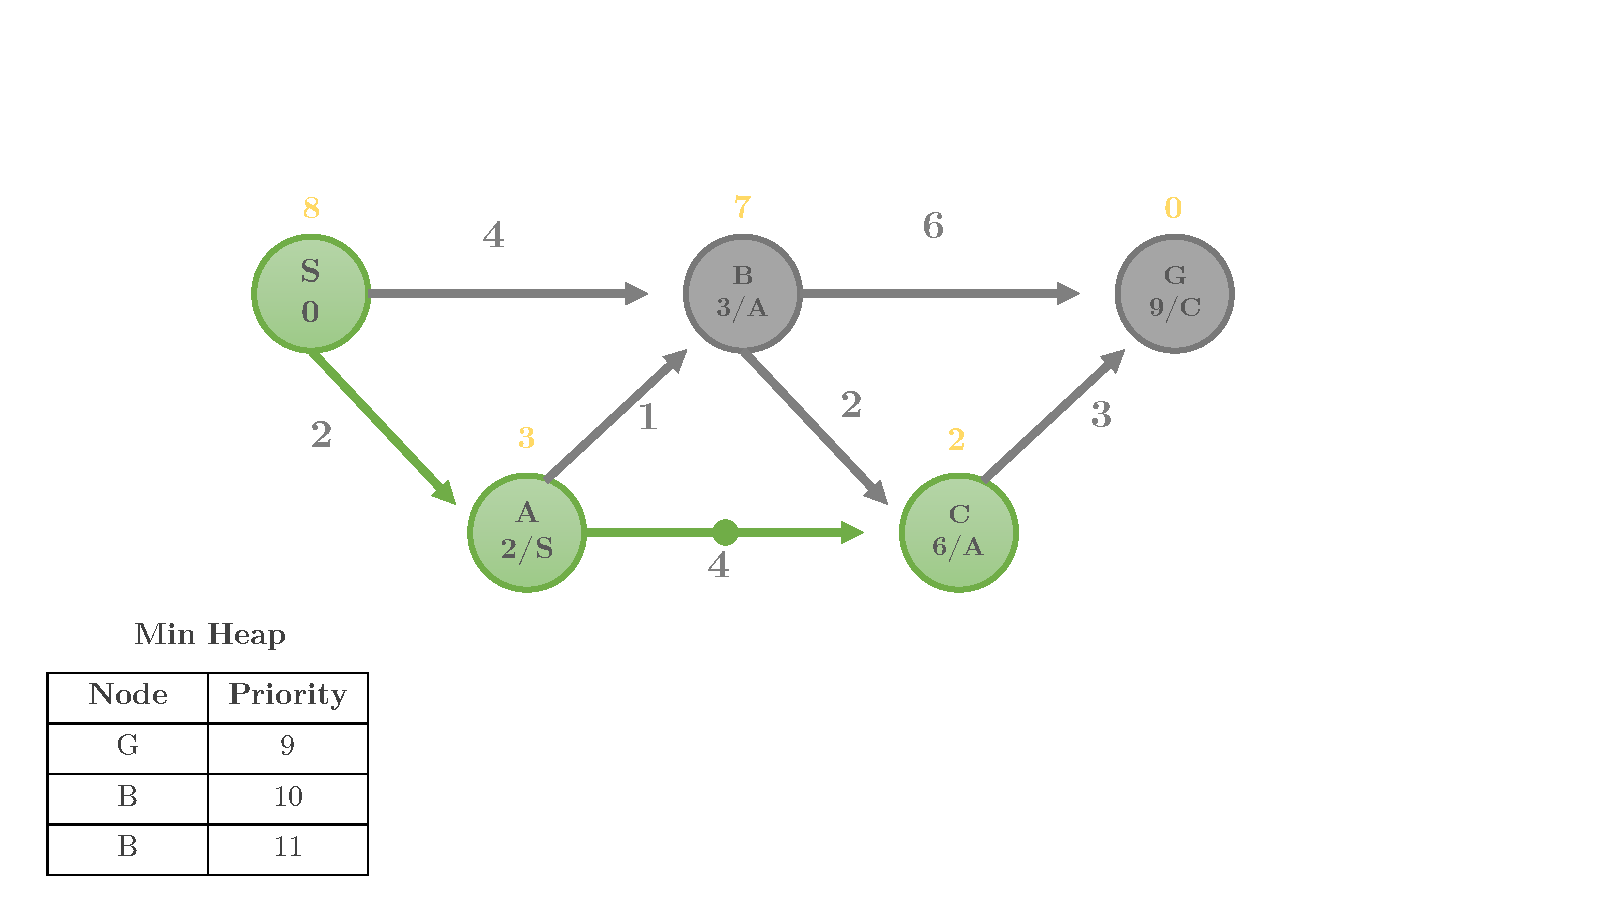
\includegraphics[width=0.9\textwidth]{heuristic1_Page4.png}
\end{center}

\begin{center}
  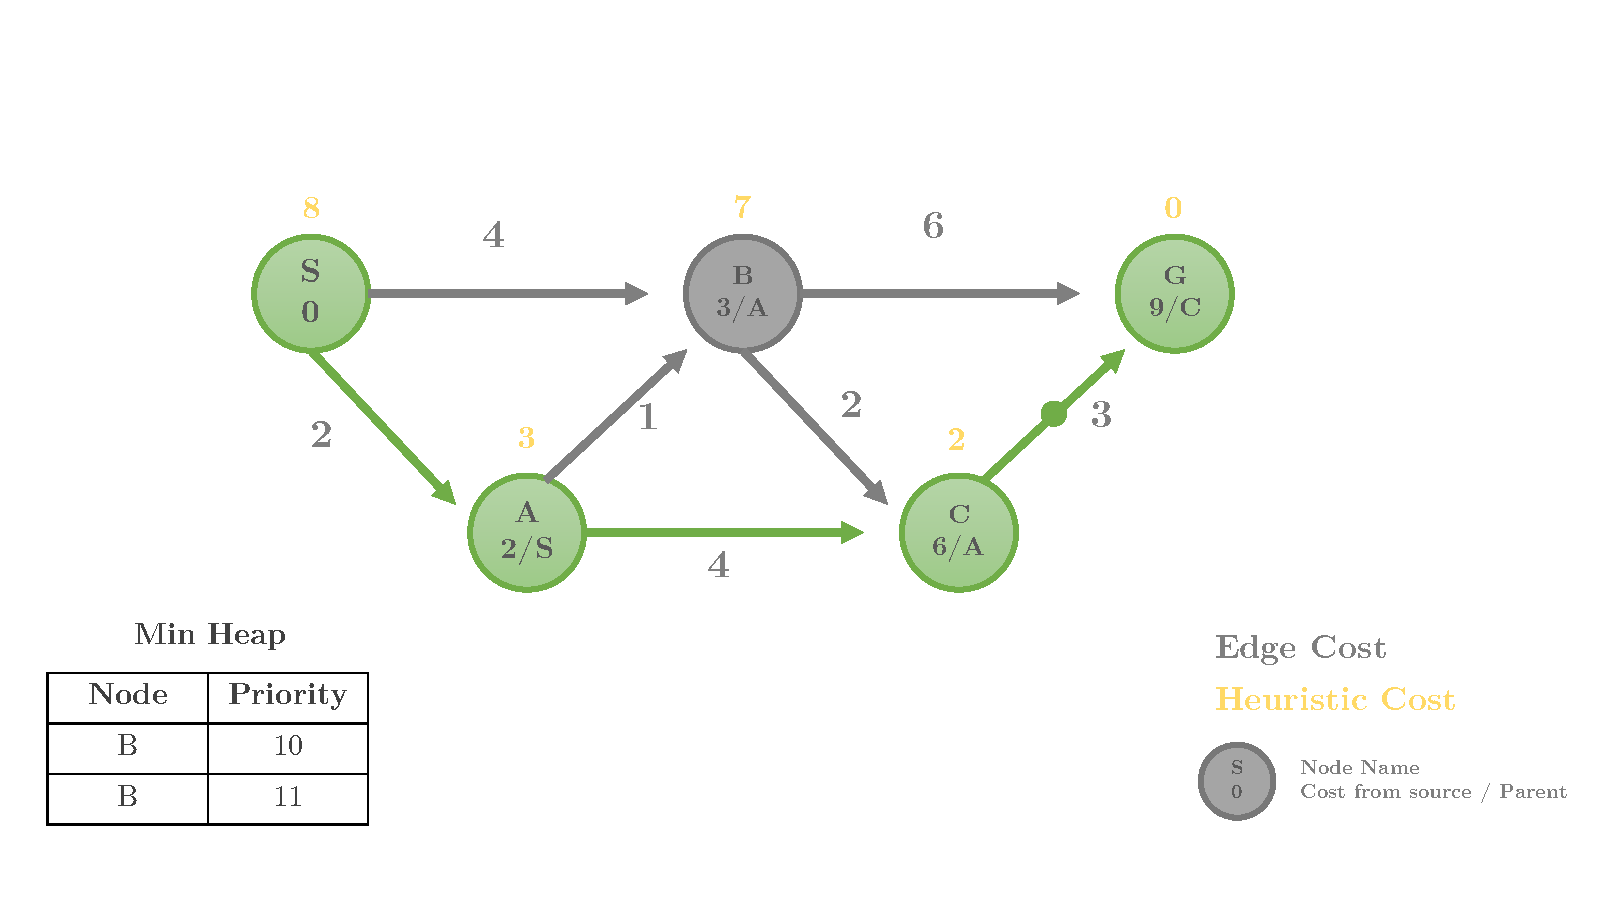
\includegraphics[width=0.9\textwidth]{heuristic1_Page5.png}
\end{center}

\begin{center}
  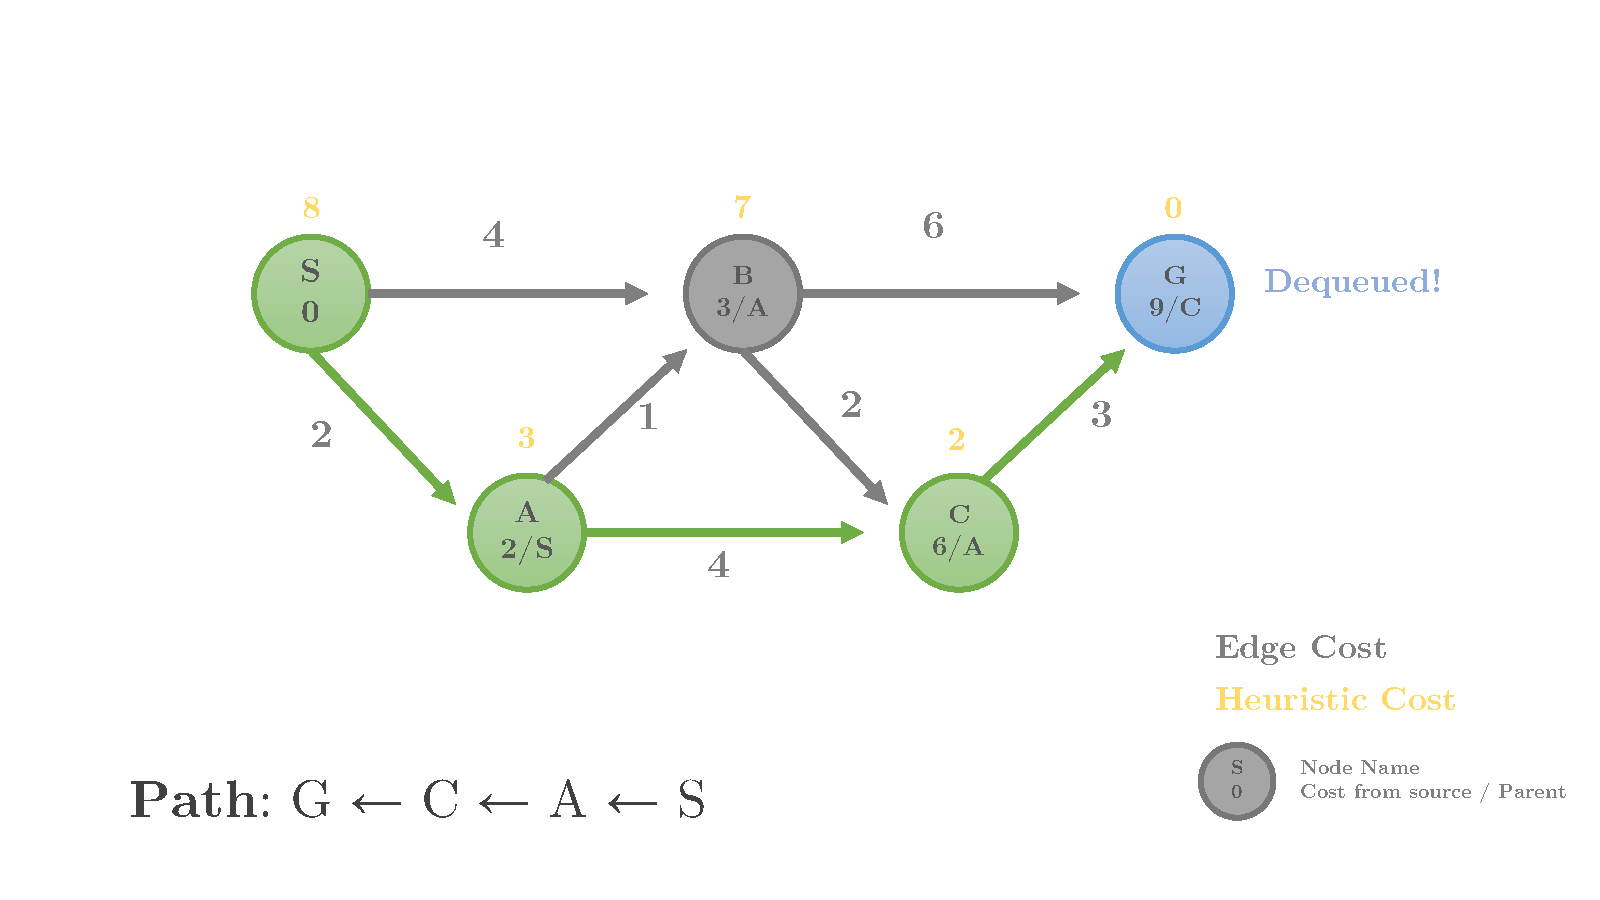
\includegraphics[width=0.9\textwidth]{heuristic1_Page6.png}
\end{center}

\noindent
\textbf{Path Cost}: 2 + 4 + 3 = 9

\pagebreak
\subsection*{Heuristic 2}

For another set of heuristics, we can simulate the search and obtain another path.

% A horizontal table containing 2 rows, one for the vertex name and the other for the heuristic cost.

\begin{table}[h]
  \centering
  \begin{tabular}{cc}
  \toprule
  \textbf{Vertex} & \textbf{Heuristic Cost} \\
  \midrule
  S & 7 \\
  A & 4 \\
  B & 5 \\
  C & 2 \\
  G & 0 \\
  \bottomrule
  \end{tabular}
\end{table}

\begin{center}
  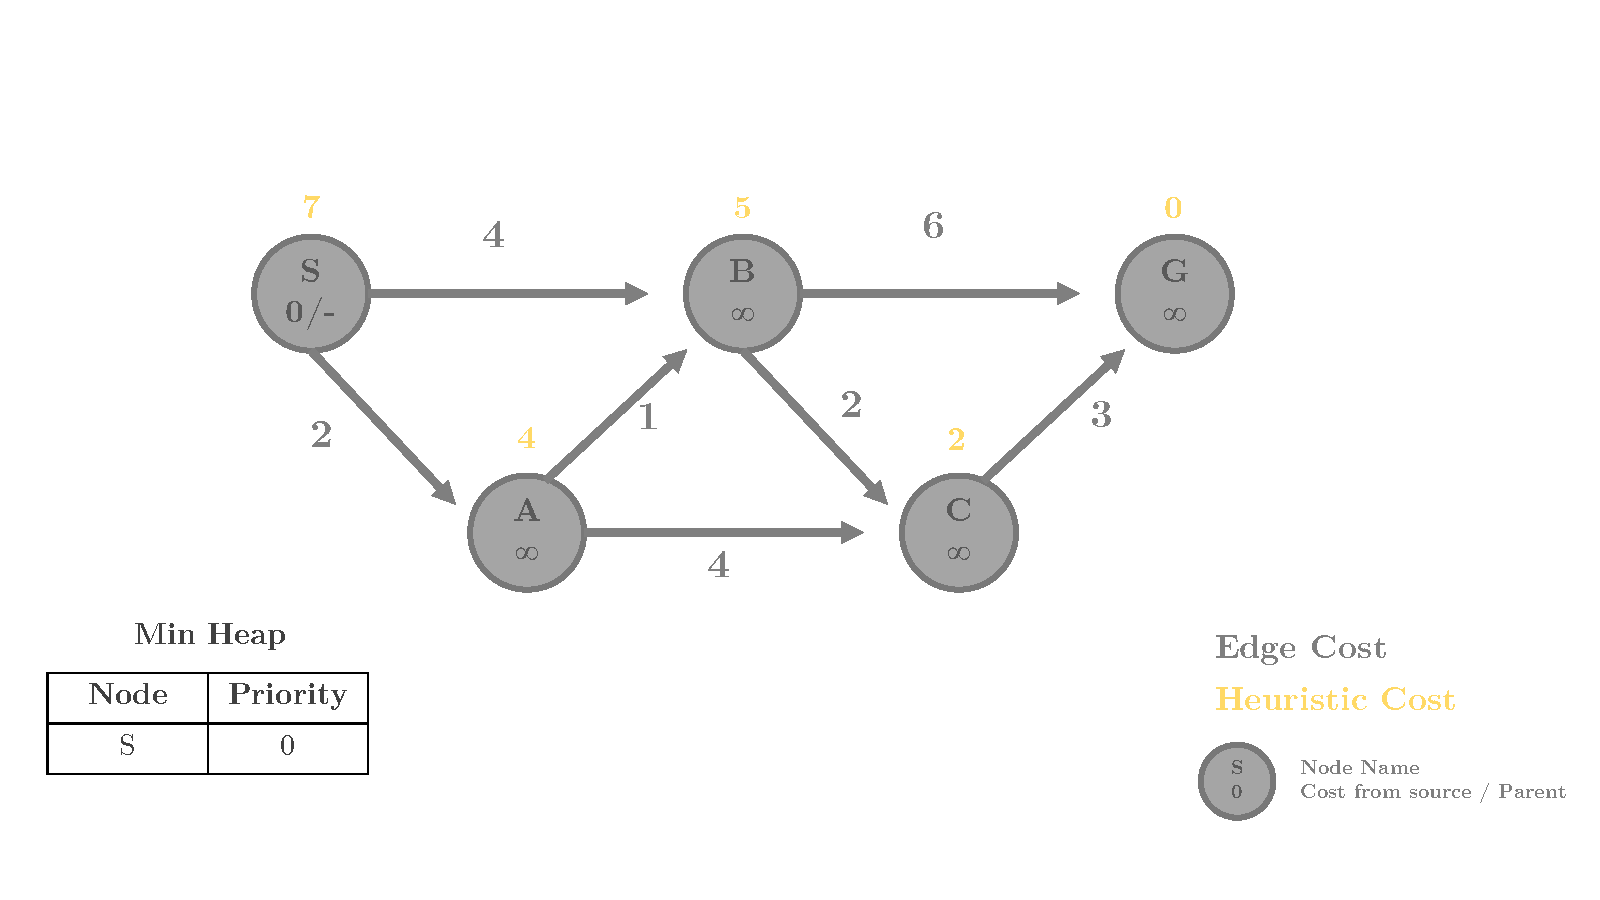
\includegraphics[width=0.9\textwidth]{heuristic2_Page1.png}
\end{center}

\begin{center}
  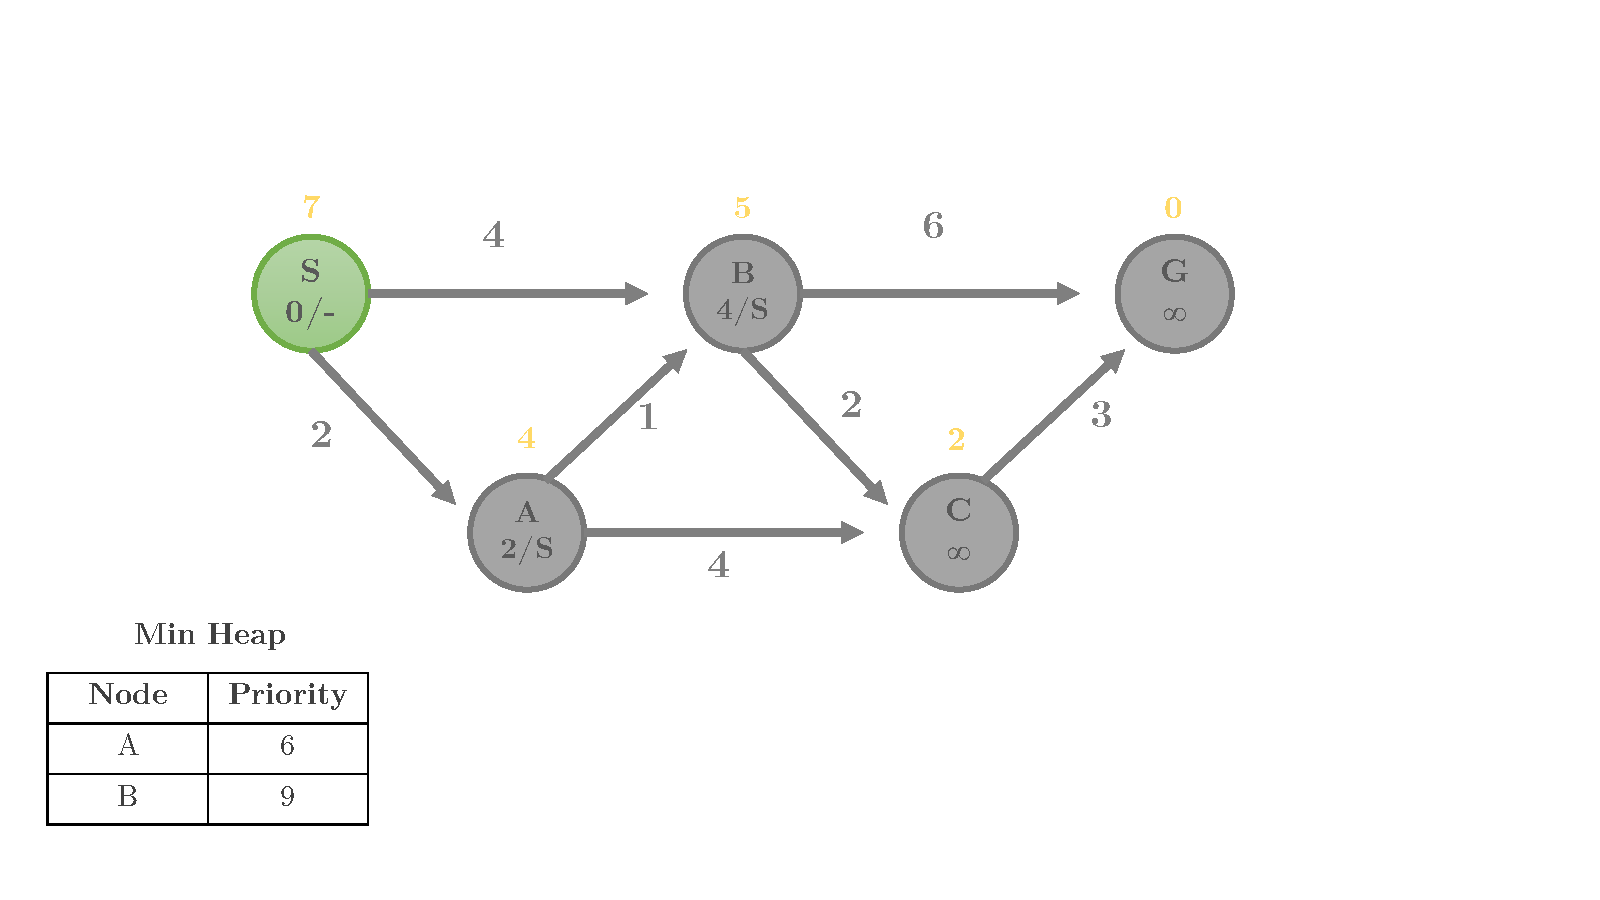
\includegraphics[width=0.9\textwidth]{heuristic2_Page2.png}
\end{center}

\begin{center}
  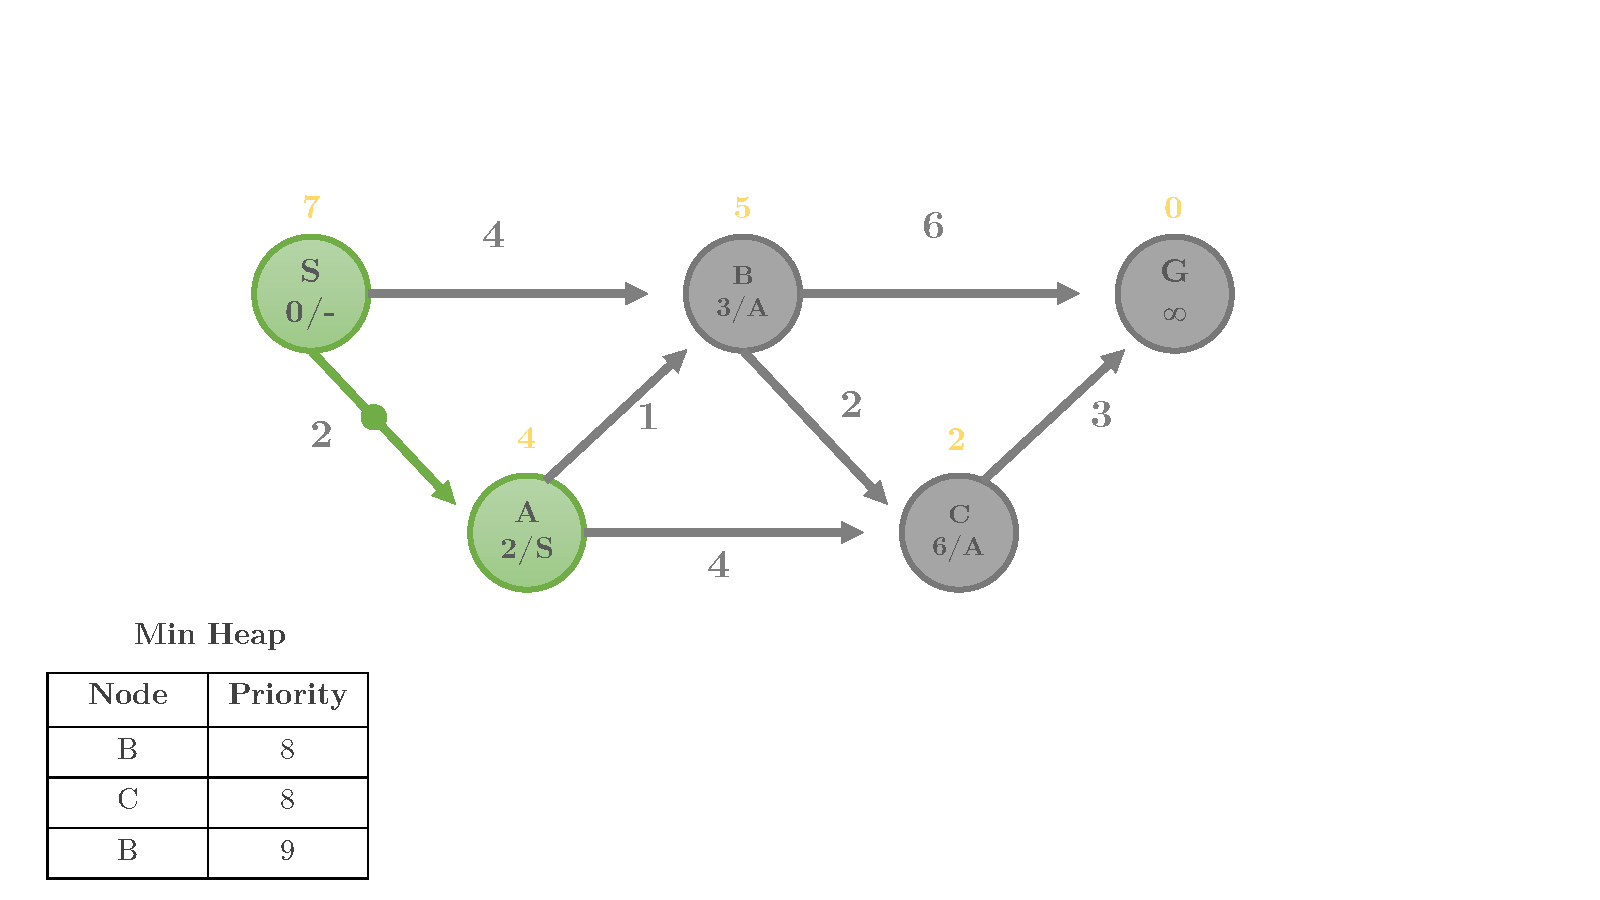
\includegraphics[width=0.9\textwidth]{heuristic2_Page3.png}
\end{center}

\begin{center}
  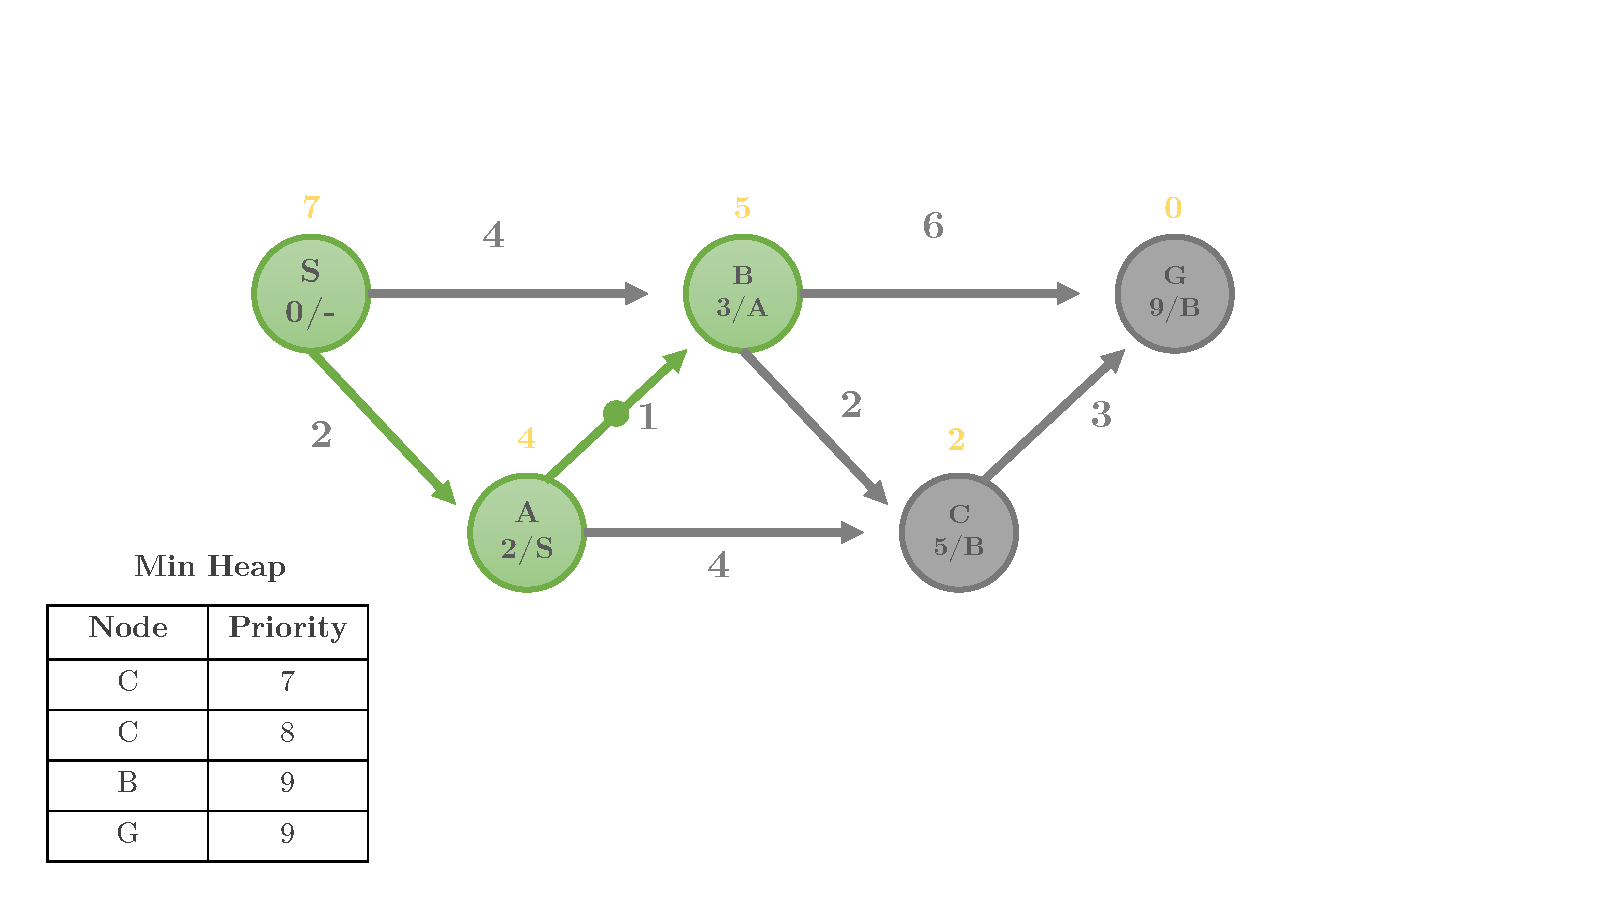
\includegraphics[width=0.9\textwidth]{heuristic2_Page4.png}
\end{center}

\begin{center}
  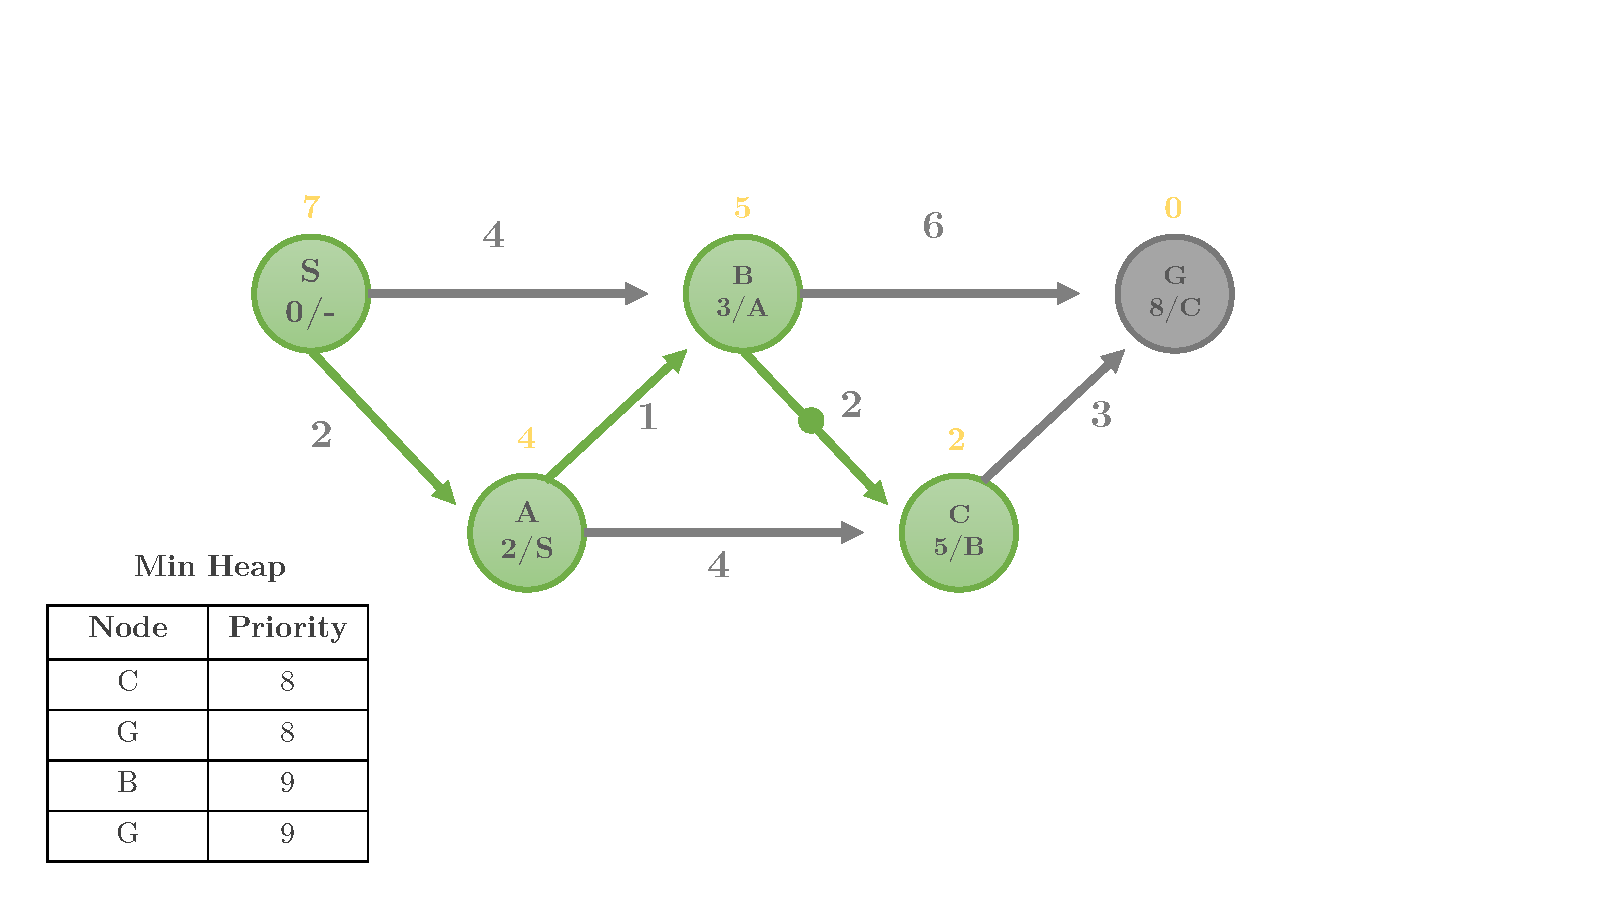
\includegraphics[width=0.9\textwidth]{heuristic2_Page5.png}
\end{center}

\begin{center}
  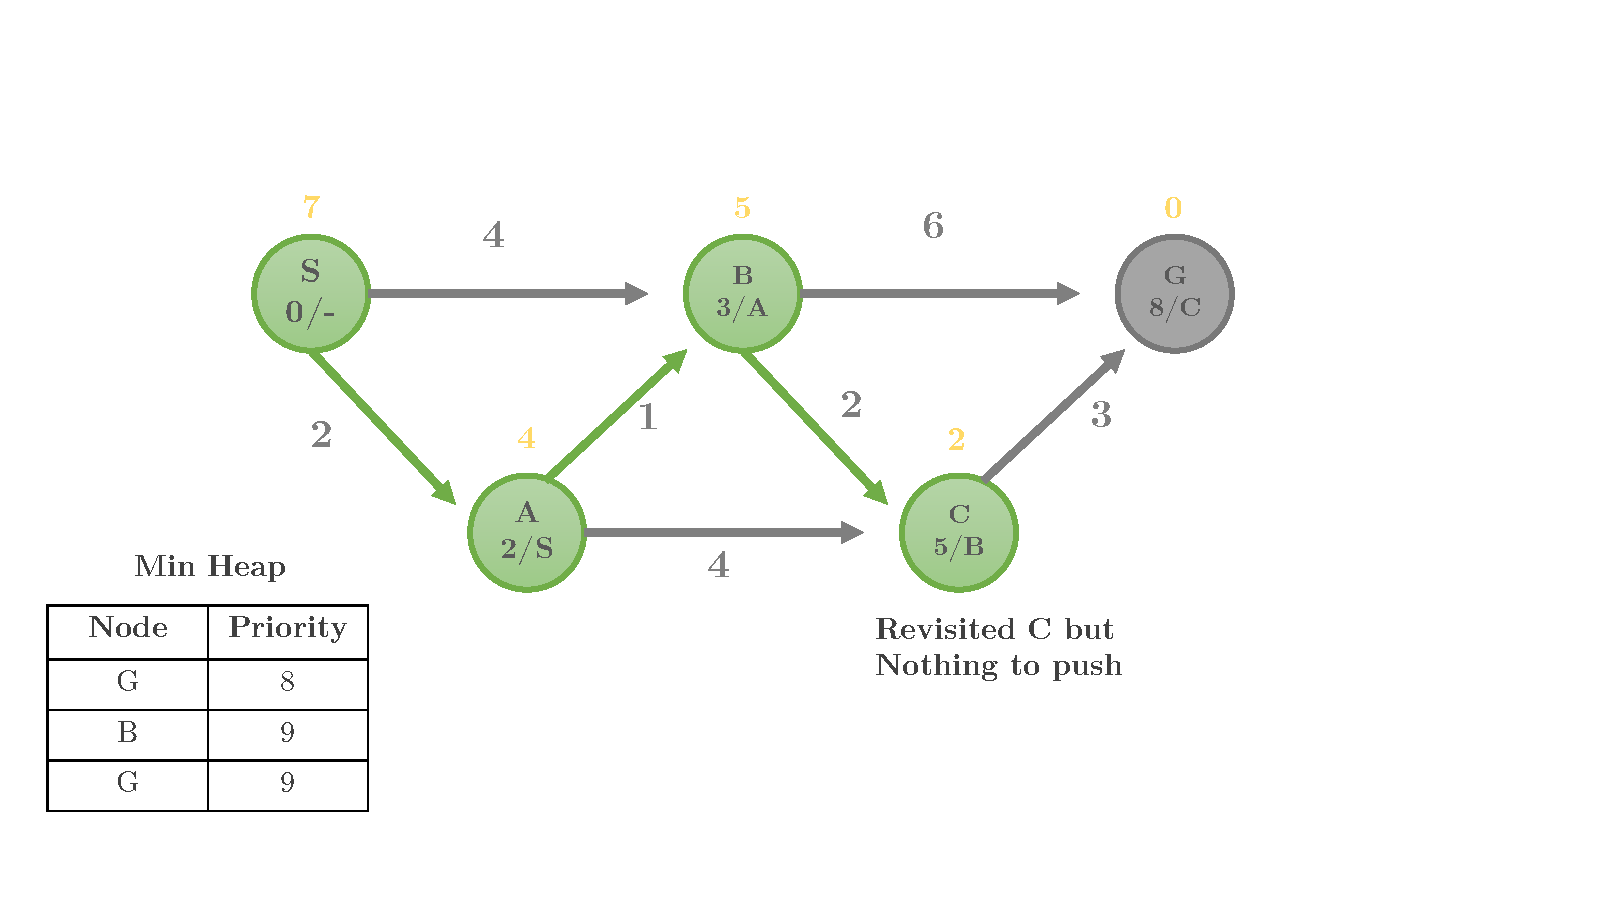
\includegraphics[width=0.9\textwidth]{heuristic2_Page6.png}
\end{center}

\begin{center}
  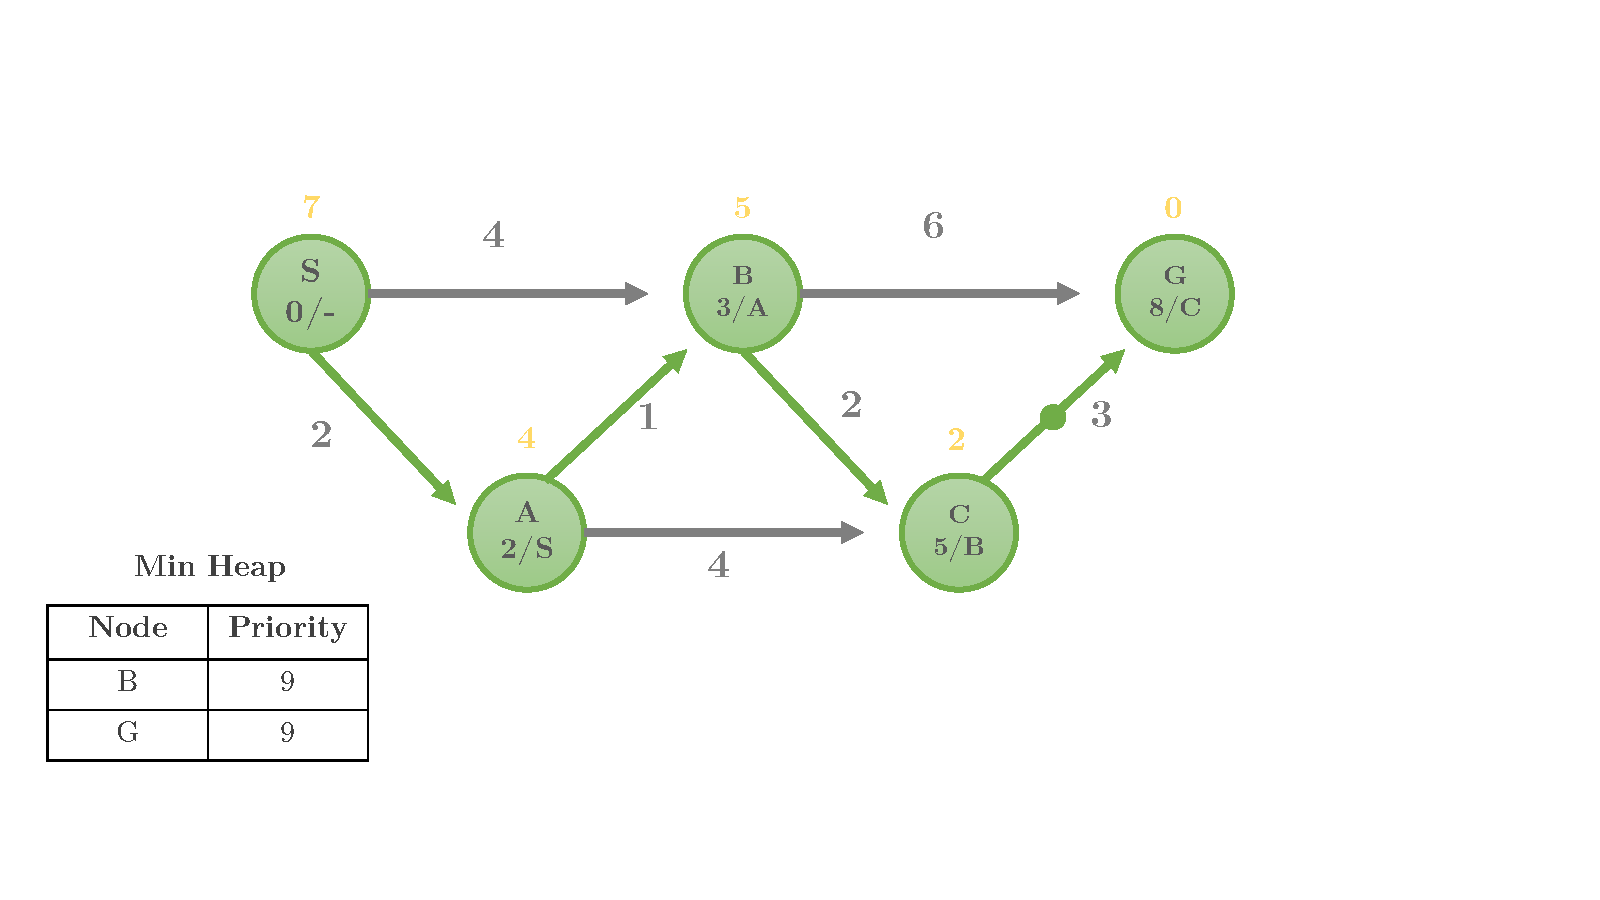
\includegraphics[width=0.9\textwidth]{heuristic2_Page7.png}
\end{center}

\begin{center}
  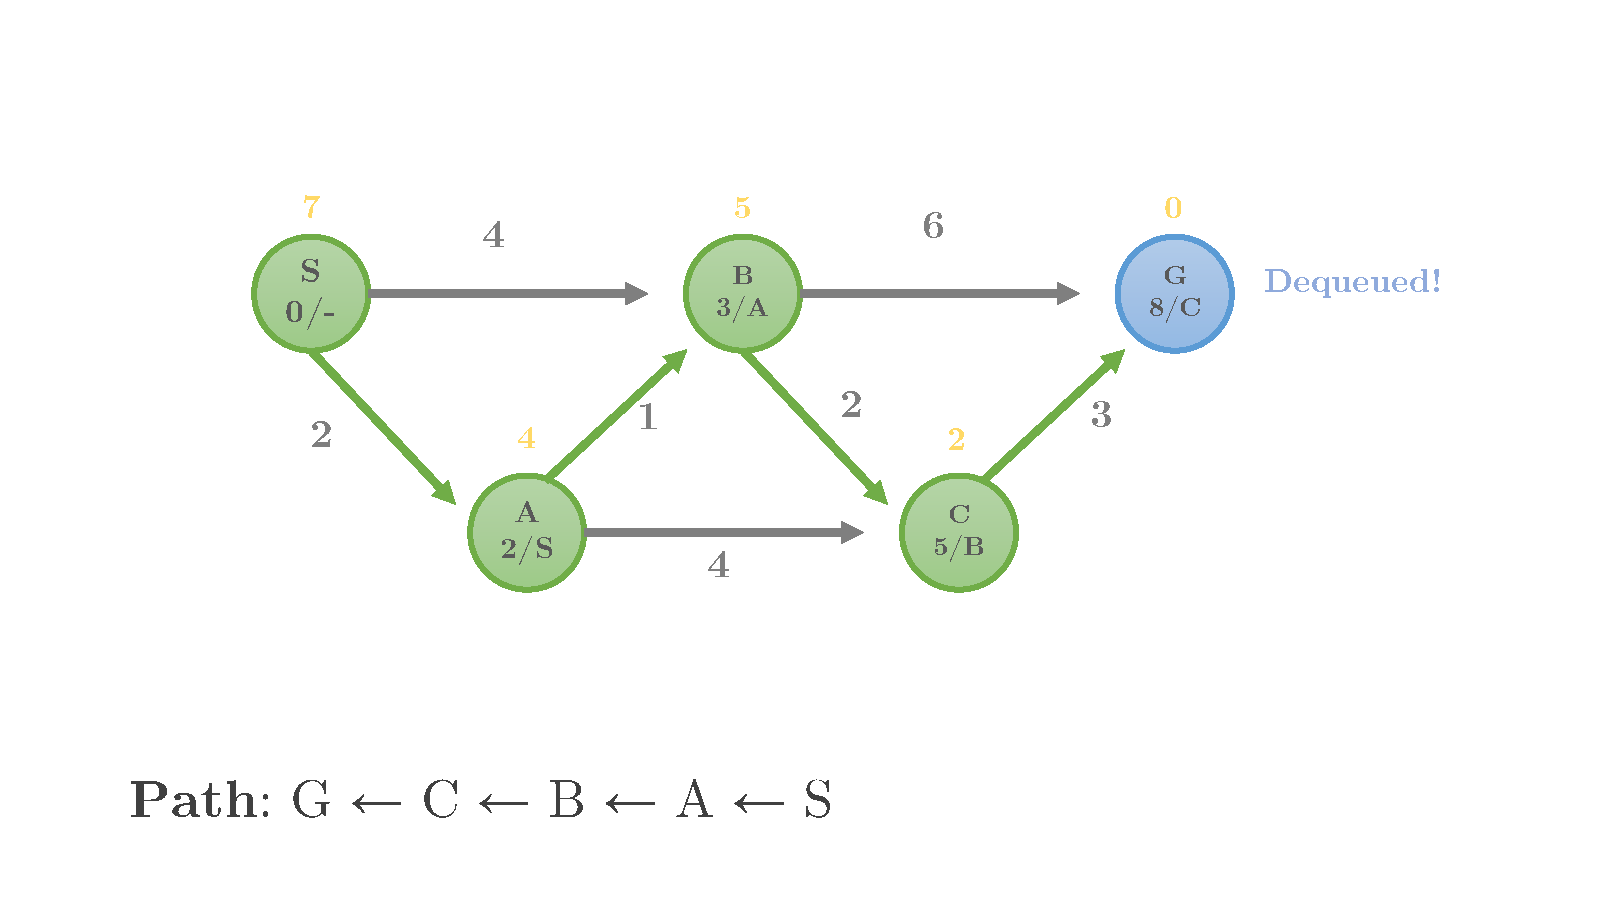
\includegraphics[width=0.9\textwidth]{heuristic2_Page8.png}
\end{center}

\noindent
\textbf{Path Cost}: 2 + 1 + 2 + 3 = 8

\pagebreak
\section*{Part B}

\subsection*{Source Code}
Attached with the report.

\subsection*{Output}
\begin{center}
  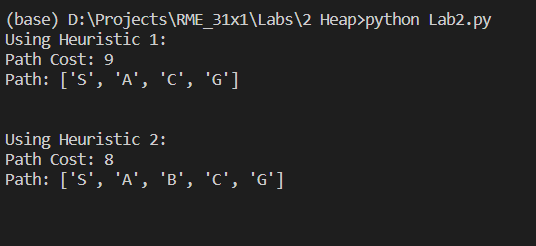
\includegraphics[width=0.9\textwidth]{Output.png}
\end{center}

\subsection*{Result Discussion}
The search result achieved using the second set of heuristics was more optimal (lower path cost) because the heuristic function was admissible. The first set of heuristics was not admissible because the heuristic cost of the vertex B (7) was greater than the actual cost of the path from G to B (6).

\end{document}
